\documentclass[]{article}

% Imported Packages
%------------------------------------------------------------------------------
\usepackage{amssymb}
\usepackage{amstext}
\usepackage{amsthm}
\usepackage{amsmath}
\usepackage{enumerate}
\usepackage{fancyhdr}
\usepackage[margin=1in]{geometry}
\usepackage{graphicx}
\usepackage{extarrows}
\usepackage{setspace}

% \renewcommand*\familydefault{\sfdefault}
% \usepackage{cmbright}
% \usepackage{helvet}
%------------------------------------------------------------------------------

% Header and Footer
%------------------------------------------------------------------------------
\pagestyle{plain}
\renewcommand\headrulewidth{0.4pt}
\renewcommand\footrulewidth{0.4pt}
%------------------------------------------------------------------------------

% Title Details
%------------------------------------------------------------------------------
\title{
  Erudite\\
  \large \emph{An educational content management system}
}

\author{
  SE 3A04: Software Design II -- Large System Design\\
  \\
  \begin{tabular}{ l l }
    Kelvin Lin*   & STUDENT-NUM \\
    Danish Khan   & STUDENT-NUM \\
    Puru Jetly    & STUDENT-NUM \\
    Terrance Yip  & STUDENT-NUM \\
    Varun Hooda   & STUDENT-NUM \\
  \end{tabular}
}

\date{}
%------------------------------------------------------------------------------

% Document
%------------------------------------------------------------------------------
\begin{document}

\maketitle


\section{Introduction}
\label{sec:introduction}
This section outlines the purpose and scope of the Erudite project; along with
definitions, acronyms and abbreviations used within this document; and finally
an overview of the contents and organization of this software requirements
document.


\subsection{Purpose}
\label{sub:purpose}
This document's purpose is to outline the engineering and business decisions
made in the design portion of the Erudite-CMS project. This document will be
used to maintain a record of project's scope, constraints, assumptions,
dependencies, functional requirements, non-functional requirements and any
other design decision made over the life of this project.

The target audience for this document are the stakeholders (Dr. Ridha Khedri,
Andrew Le Clair and Michael Liut), and any current or future architects,
designers and developers of this project.


\subsection{Scope}
\label{sub:scope}
This project will produce the following software products:
\begin{itemize}
  \item \underline{Android} Client Application
  \item Back-end Web Server
  \item Back-end Database Server
\end{itemize}

\noindent The aforementioned products preform the following:
\begin{itemize}
  \item Provide users with a graphical client-side application for creating,
    modifying and viewing server hosted content.
  \item Provide a means of retrieving and sending data between the front-end
    client and back-end web server.
  \item Provide a means of persistent storage and retrieval of content.
\end{itemize}

\noindent The aforementioned products do not preform the following:
\begin{itemize}
  \item Generate content.
\end{itemize}

\noindent These software products will combine to provide a content management system for
teachers and students in an educational environment. Benefits include quick
accesses to educational content, efficient management of content, portability
and ease of access to content, and Ease of grading of assessable contents
(quizzes). The goals include providing students and teachers with a smilier
interface to access and add content, all the while reducing any additional
overhead of maintaining a system, and providing easy accessibility to all
users.



\subsection{Definitions, Acronyms, and Abbreviations}
\label{sub:definitions_acronyms_and_abbreviations}
\begin{description}
  \item [Access Rights] See Permissions.

  \item [Android] a mobile operating system developed by Google Inc.  primarily
    for touchscreen mobile devices.

  \item [Classroom Operations] The set of typical actions performed in a
    classroom.

  \item [CMS] A system capable of hosting, managing and delivering digital
    content to user.

  \item [LMS] Learning Management System. A specific instance of a Content
    Management System with am emphasis on educational or learning materials and
    institutions.

  \item [Mechanism of Assessment] Assignments, Quizzes, and other ways of
    assessing and evaluating a students knowledge

  \item [Metric of Success] Means of measuring a student's knowledge (grades,
    points, stars, percentage, etc.)

  \item [Permissions] The allowed set of actions a user is able to perform.

  \item [Smartphone] An embedded electronic device capable of serving as a
    general purpose computer in addition to providing mobile telephone
    functionality such as phone calls and text messaging.

  \item [Teaching Methods] Ways of teaching including but not limited to
    assignments, examinations and tests.

  \item [User Role] Categorization of the user into a set of possible
    institutional roles (administration, teacher, student).
\end{description}


\subsection{References}
\label{sub:references}
void


\subsection{Overview}
\label{sub:overview}
The rest of this documents contains detailed descriptions of this projects
design decisions: assumptions, functionality, functional requirements and
non-functional requirements.

The other sections are organized into logical subsections. Specifically, section
2 outlines the overall product description with various subsections. Then the
following sections list the requirements. The functional requirements are
organized by business events and viewpoints. Non-functional requirements are
organized, also, into logical subsections.


% End Section


\section{Overall Description}
\label{sec:overall_description}
% Begin Section

This section of the SRS should describe the general factors that affect the
product and its requirements. It does not state specific requirements; it
provides a background for those requirements and makes them easier to
understand.

\subsection{Product Perspective}
\label{sub:product_perspective}
% Begin SubSection
Plan 6 is a distributed learning management system designed to facilitate
teachers and students with everyday \underline{classroom operations}. Plan 6 is
a distributed, self-contained system with several components running on
different end-user devices. Plan 6 is akin to other learning management
systems, such as McMaster's Avenue2Learn; however, Plan 6 will focus on
providing a Learning Management System for early learners and educators with
low levels of technical expertise.

A block diagram denoting the major components of system as well as their
external interfaces follow:

\begin{center}
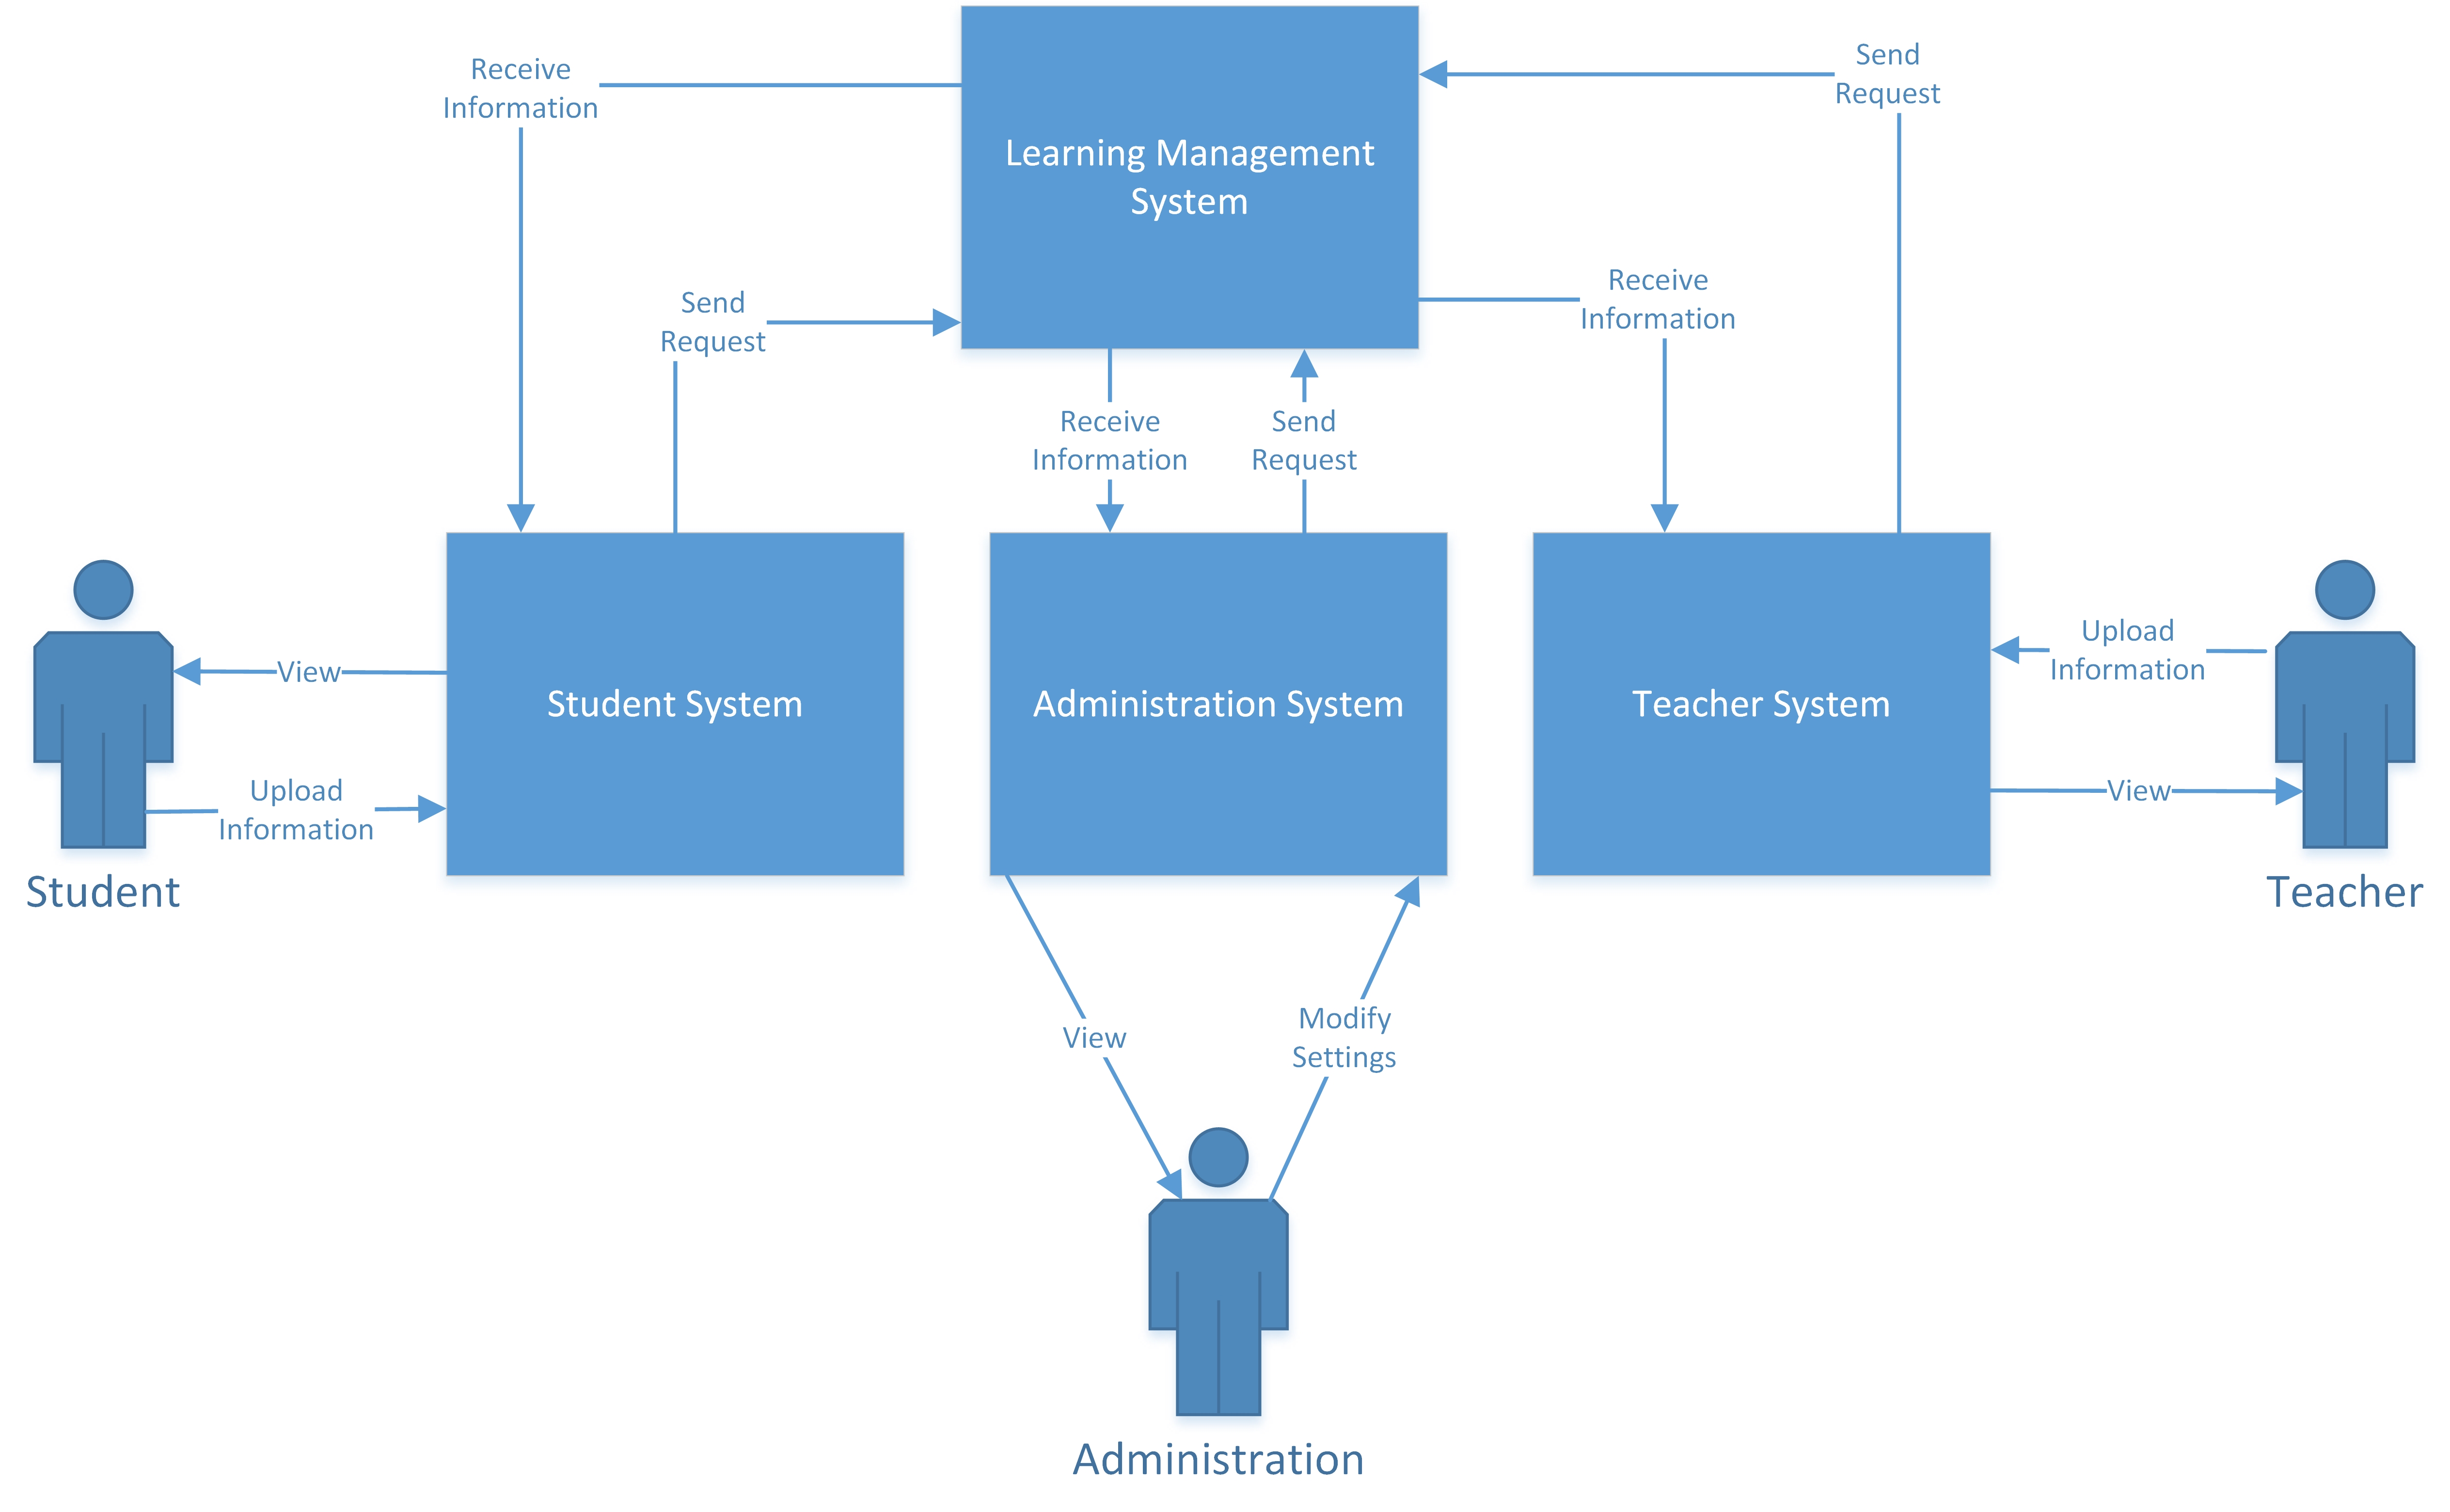
\includegraphics[scale=0.7]{A1_Assets/2-1_Product_Perspective_Diagram.jpg}
\end{center}

% End SubSection

\subsection{Product Functions}
\label{sub:product_functions}
% Begin SubSection
Edurite-LMS is designed to facilitate students, teachers, and administration
with common classroom operations.

As a \underline{LMS}, Edurite-LMS will allow teachers to upload a variety of documents for
the purpose of education. Teachers are then able to set the duration that the
documents are available, as well as the the \underline{access rights} users
have over the document.

Moreover, Edurite-LMS will allow teachers to create virtual mechanisms of
assessment including but not limited to quizzes, and electronic assignment
submission boxes. With virtual quizzes, teachers will be allowed to create their
own questions and solutions.

Teachers will also be able to configure settings related to these mechanisms of
assessment including but not limited to the availability of the mechanism,
functionalities available while users are participating in the mechanism of
assessment, and the assessment scheme associated with the mechanism.

The LMS will also allow teachers to enter success metrics for each student. If
instructed to do so, the LMS will also be able to automatically assess students
based on primitive assessment schemes provided by the teacher.

Edurite-LMS will allow teachers to view statistics associated with each
\underline{mechanism of assessment}. It will create visualizations of data generated from
the results of the assessment scheme and display them to the teacher. Statistics
to be displayed to the teacher include but is not limited to the statistical
mean, the statistical mode, the variance, the standard deviation, the point
biserial, and the discrimination index.

On the other hand, Edurite-LMS will allow students to view documents uploaded by
the teacher. The students will be able to save a copy of the document if it is
allowed by the teacher.

Moreover, Edurite-LMS will allow students to complete virtual mechanisms of
assessments created by their teacher. The LMS will allow students to submit the
appropriate information in order to successfully complete the mechanism of
assessment. The LMS will show the student a \underline{metric of success} when
authorized by the teacher.

Finally, Edurite-LMS will allow administration to add or remove students from
certain domains. The LMS will allow administration to modify the
\underline{user roles} and to control what \underline{permissions} each role has
over the system.
% End SubSection

\subsection{User Characteristics}
\label{sub:user_characteristics}
% Begin SubSection
Edurite-LMS is intended for 3 primary groups of users: teachers, students, and
administration.

Teachers are assumed to be adult users with the functional capacity of an
average person who is between the ages of 16 and 80. Teachers are assumed to be
fluent in written English, and have at least a basic understanding of
mathematics and statistics. Moreover, teachers are assumed to have a strong
understanding of \underline{teaching methods}; however, teachers are not assumed to be
well-versed in technology. Teachers should know how to use an Android platform
- including typing and selecting elements on the screen - however, they are not
expected to know how to know advanced features of the phone.

Students are assumed to be child users of ages 6 to 13, who are enrolled in a
Canadian, American, or equivalent elementary school. Students are assumed to
understand basic written English at the Ontario Senior Kindergarten/Grade 1
level. Students are expected to have vision and are able to use the basic
functions of the Android platform, albeit at a lower level than teachers and
administrations. At a minimum, students are assumed to know how to select
elements on the screen. No other prior knowledge is assumed of the student.

The administration is assumed to be adult users with the functional capacity of
an average person who is between the ages of 16 to 80. The administration is
assumed to be fluent in written English, and have a good understanding of
mathematics and statistics. The administration is also assumed to have basic
computer knowledge, including basic troubleshooting, IT, and data entry skills.
The administration is assumed to have an intermediate understanding of common
Android platform usage, and are able to preform more advanced tasks such as
set-up, installation, and troubleshooting on such platforms.
% End SubSection

\subsection{Constraints}
\label{sub:constraints}
% Begin SubSection
The application must run on the native Android platform, as per the project
specifications provided.
% End SubSection

\subsection{Assumptions and Dependencies}
\label{sub:assumptions_and_dependencies}
% Begin SubSection
It is assumed that the school using the system will have the necessary infrastructure to support the system. The school will provide the required hardware in order to reasonably ensure the security of the data, and to handle the data capacity requirement.

Moreover, it is assumed that each user will have access to an Android platform that is internet enabled.
% End SubSection

\subsection{Apportioning of Requirements}
\label{sub:apportioning_of_requirements}
% Begin SubSection
This section is void.
% End SubSection

% End Section

\section{Functional Requirements}
\label{sec:functional_requirements}
	% Begin Section
	% This section of the SRS should contain all of the software requirements to a level of detail sufficient to enable designers to design a system to satisfy those requirements, and testers to test that the system satisfies those requirements. Throughout this section, every stated requirement should be externally perceivable by users, operators, or other external systems. These requirements should include at a minimum a description of every input (stimulus) into the system, every output (response) from the system, and all functions performed by the system in response to an input or in support of an output.

	% You normally have two options for organizing your functional requirements:
	%\begin{enumerate}
	%	\item Organize first by \emph{business events}, then by \emph{viewpoints}
	%	\item Organize first by \emph{viewpoints}, then by \emph{business events}
	%\end{enumerate}
	%Choose the one which makes the most sense.

% For example, if you wish to organization by business events:

% TEACHER BUSINESS EVENTS (5)

\begin{enumerate}[{BE}1.]
	\item A teacher creates a course and owns it or deletes an existing course the teacher owns.
	\begin{enumerate}[{VP1}.1]
		\item Student Viewpoint
			\begin{enumerate}
				\item Students must be able to enroll in an existing course owned by the teacher provided the course is set visible.
			\end{enumerate}
		\item Teacher Viewpoint
			\begin{enumerate}
				\item A teacher must be able to choose to unenroll a student from a course that the teacher owns.
				\item A teacher is not enrolled in a course.
			\end{enumerate}
		\item Parent Viewpoint
			\begin{enumerate}
				\item \*\*\*\*\* Should a parent wish to see course progress or student performance, they are required to use the child's student account.
			\end{enumerate}
		\item School Administration Viewpoint
			\begin{enumerate}
				\item The school administration  choose to either allow students and teachers to create their own accounts, or create accounts for all students and teachers.
			\end{enumerate}
		\item Information Technology Team Viewpoint
			\begin{enumerate}
				\item None
			\end{enumerate}
		\item Government \& School Board Viewpoint
			\begin{enumerate}
				\item All courses, course content, and any teacher student communication
          held on the \underline{CMS} must be made visible to the School Board.
			\end{enumerate}
	\end{enumerate}

	\item A teacher adds non-evaluational, manual-evaluational or automated-evaluational content to a course owned by that teacher.
	\begin{enumerate}[{VP1}.1]
		\item Student Viewpoint
			\begin{enumerate}
				\item A student enrolled in a course must be able to view any content within the course provided the content is set visible by the owner of that course.
				\item A student must be able to submit an \textbf{student assignment}; a piece of content uploaded in response to a manual-evaluational content provided the manual-evaluational content is set visible by the owner of that course.
				\item A student must be able to submit an automated evaluational content provided it is set visible by the owner of that course.
			\end{enumerate}
		\item Teacher Viewpoint
			\begin{enumerate}
				\item Non-evaluational content is any content for which students are given only the option to view the content.
				\item Manual-evaluational content is any content where, in addition to viewing, students must be able to post their own content in response, called a submitted assignment, to the content posted by the teacher.
				\item Automated-evaluational content is any content that when accessed by students, allows students to interact with that content and the result of their interaction is marked by a previously defined success criteria defined by the owner of the course.
				\item The student's performance in the exploration of automated-evaluational content is recorded and saved for future reference by the student and the teacher.
			\end{enumerate}
		\item Parent Viewpoint
			\begin{enumerate}
				\item None
			\end{enumerate}
		\item School Administration Viewpoint
			\begin{enumerate}
				\item None
			\end{enumerate}
		\item Information Technology Team Viewpoint
			\begin{enumerate}
				\item None
			\end{enumerate}
		\item Government \& School Board Viewpoint
			\begin{enumerate}
				\item None
			\end{enumerate}
	\end{enumerate}

	\item A teacher views a submitted student assignment.
	\begin{enumerate}[{VP2}.1]
		\item Student Viewpoint
			\begin{enumerate}
				\item Students must be able to submit assignments multiple times in response to a manual-evaluational content posted by the course owner.
			\end{enumerate}
		\item Teacher Viewpoint
			\begin{enumerate}
				\item A teacher must be able to assign either a numerical or letter grade to the assignment.
			\end{enumerate}
		\item Parent Viewpoint
			\begin{enumerate}
				\item None
			\end{enumerate}
		\item School Administration Viewpoint
			\begin{enumerate}
				\item None
			\end{enumerate}
		\item Information Technology Team Viewpoint
			\begin{enumerate}
				\item None
			\end{enumerate}
		\item Government \& School Board Viewpoint
			\begin{enumerate}
				\item None
			\end{enumerate}
	\end{enumerate}

	\item A teacher adds a quiz or deletes an existing quiz.
	\begin{enumerate}[{VP2}.1]
		\item Student Viewpoint
			\begin{enumerate}
				\item Quizzes are made visible to students only if they are set visible by the owner of the course.
			\end{enumerate}
		\item Teacher Viewpoint
			\begin{enumerate}
				\item A quiz is set visible for a time period specified by the owner of the course. A quiz is set not visible otherwise.
			\end{enumerate}
		\item Parent Viewpoint
			\begin{enumerate}
				\item None
			\end{enumerate}
		\item School Administration Viewpoint
			\begin{enumerate}
				\item None
			\end{enumerate}
		\item Information Technology Team Viewpoint
			\begin{enumerate}
				\item None
			\end{enumerate}
		\item Government \& School Board Viewpoint
			\begin{enumerate}
				\item None
			\end{enumerate}
	\end{enumerate}

	\item The owner of a course specifies a time period for which course material, course assignments, course assessments or a course is set visible for all enrolled students.
	\begin{enumerate}[{VP2}.1]
		\item Student Viewpoint
			\begin{enumerate}
				\item A student is unenrolled from a course that is set not visible.
				\item An enrolled student must not be able to view course material, course assignments, or course assessment content or course which is not made visible by the owner of the course.
			\end{enumerate}
		\item Teacher Viewpoint
			\begin{enumerate}
				\item A teacher must be able to permanently remove a piece of content from a course owned by them.
			\end{enumerate}
		\item Parent Viewpoint
			\begin{enumerate}
				\item None
			\end{enumerate}
		\item School Administration Viewpoint
			\begin{enumerate}
				\item None
			\end{enumerate}
		\item Information Technology Team Viewpoint
			\begin{enumerate}
				\item None
			\end{enumerate}
		\item Government \& School Board Viewpoint
			\begin{enumerate}
				\item None
			\end{enumerate}
	\end{enumerate}

% STUDENT BUSINESS EVENTS (4)

	\item A student enrolls within a course that is set visible by the owner of that course.
	\begin{enumerate}[{VP2}.1]
		\item Student Viewpoint
			\begin{enumerate}
				\item A student must be able view all courses to which they are enrolled.
				\item A student must not be able to self withdraw from a course in which he or she is enrolled.
				\item A student that is dismissed from a course is not longer enrolled in that course.
				\item A student whom is not enrolled in a course has no access to content found within that course.
			\end{enumerate}
		\item Teacher Viewpoint
			\begin{enumerate}
				\item A teacher must be able to dismiss an enrolled student from a course owned by the teacher.
			\end{enumerate}
		\item Parent Viewpoint
			\begin{enumerate}
				\item None
			\end{enumerate}
		\item School Administration Viewpoint
			\begin{enumerate}
				\item None
			\end{enumerate}
		\item Information Technology Team Viewpoint
			\begin{enumerate}
				\item None
			\end{enumerate}
		\item Government \& School Board Viewpoint
			\begin{enumerate}
				\item None
			\end{enumerate}
	\end{enumerate}

	\item A student checks all the grades assigned to them for all submitted student assignments and student quizzes for all courses in which the student is enrolled.
	\begin{enumerate}[{VP2}.1]
		\item Student Viewpoint
			\begin{enumerate}
				\item None
			\end{enumerate}
		\item Teacher Viewpoint
			\begin{enumerate}
				\item None
			\end{enumerate}
		\item Parent Viewpoint
			\begin{enumerate}
				\item None
			\end{enumerate}
		\item School Administration Viewpoint
			\begin{enumerate}
				\item None
			\end{enumerate}
		\item Information Technology Team Viewpoint
			\begin{enumerate}
				\item None
			\end{enumerate}
		\item Government \& School Board Viewpoint
			\begin{enumerate}
				\item None
			\end{enumerate}
	\end{enumerate}

	\item A student submits a file in response to a course assignment only if the course assignment was made visible to all students and if a submission was allowed for that course assignment.
	\begin{enumerate}[{VP2}.1]
		\item Student Viewpoint
			\begin{enumerate}
				\item
			\end{enumerate}
		\item Teacher Viewpoint
			\begin{enumerate}
				\item A
			\end{enumerate}
		\item Parent Viewpoint
			\begin{enumerate}
				\item None
			\end{enumerate}
		\item School Administration Viewpoint
			\begin{enumerate}
				\item None
			\end{enumerate}
		\item Information Technology Team Viewpoint
			\begin{enumerate}
				\item None
			\end{enumerate}
		\item Government \& School Board Viewpoint
			\begin{enumerate}
				\item None
			\end{enumerate}
	\end{enumerate}

	\item A student must be able to view all course assignments within a course in which they are enrolled provided that the owner of the course has marked them visible to be all students.
	\begin{enumerate}[{VP2}.1]
		\item Student Viewpoint
			\begin{enumerate}
				\item None
			\end{enumerate}
		\item Teacher Viewpoint
			\begin{enumerate}
				\item None
			\end{enumerate}
		\item Parent Viewpoint
			\begin{enumerate}
				\item None
			\end{enumerate}
		\item School Administration Viewpoint
			\begin{enumerate}
				\item None
			\end{enumerate}
		\item Information Technology Team Viewpoint
			\begin{enumerate}
				\item None
			\end{enumerate}
		\item Government \& School Board Viewpoint
			\begin{enumerate}
				\item None
			\end{enumerate}
	\end{enumerate}

% SCHOOL ADMINISTRATION BUSINESS EVENTS (4)

	\item The school administration adds a Teacher or a Student account or deletes an existing Teacher or Student account.
	\begin{enumerate}[{VP1}.1]
		\item Student Viewpoint
			\begin{enumerate}
				\item The student recieves a Student ID and password to access their personal if a new student account.
				\item The student must choose a new password upon first signing into the system.
				\item If a student account is deleted, they are unenrolled from all courses. Furthermore, all grades, submitted student assignments and submitted student assessments are also deleted.
			\end{enumerate}
		\item Teacher Viewpoint
			\begin{enumerate}
				\item The teacher recieves a Teacher ID and password to access their personal teacher account.
				\item The teacher must choose a new password upon first signing into the system.
				\item If a teacher account is deleted, students enrolled in courses owned by the teacher are unenrolled from the courses owned by that teacher. Furthermore, all courses owned by them are also deleted, and all course material, course assignment and course assessment content within courses owned by that teacher are also deleted.
			\end{enumerate}
		\item Parent Viewpoint
			\begin{enumerate}
				\item Should the parent require access to their child's account, the child is expected to login through their student account to allow the parent to inspect course progress or student performance.
			\end{enumerate}
		\item School Administration Viewpoint
			\begin{enumerate}
				\item The School Administration must be able to create a set of usernames and passwords from a CSV file.
				\item The passwords for the students and teachers are generated as follows DDMMYYYY where DDMMYYYY refers to the date of birth of the student or teacher.
			\end{enumerate}
		\item Information Technology Team Viewpoint
			\begin{enumerate}
				\item None
			\end{enumerate}
		\item Government \& School Board Viewpoint
			\begin{enumerate}
				\item It is expected that the responsibilities of monitoring communication is forwarded to the school administration. All enquiries are assumed to be forwarded to the school administration that are expected to use special access privileges to investigate issues regarding content or communication.
				\item Should any content maliagn against board policies, the school administration are given access and privileges to hide, remove or track the origin of a piece of content or course.
			\end{enumerate}
	\end{enumerate}

	\item The school administration views a course owned by a Teacher or deletes an existing course owned by a Teacher.
	\begin{enumerate}[{VP1}.1]
		\item Student Viewpoint
			\begin{enumerate}
				\item A student is unenrolled from a course that is deleted.
			\end{enumerate}
		\item Teacher Viewpoint
			\begin{enumerate}
				\item A teacher does not own a deleted course.
			\end{enumerate}
		\item Parent Viewpoint
			\begin{enumerate}
				\item None
			\end{enumerate}
		\item School Administration Viewpoint
			\begin{enumerate}
				\item A course is deleted when all students enrolled in that course are unenrolled from that course and all course material, course assignment, course assessment, student assignment, and student assessment content within that course is also deleted.
				\item The school administration account is given a warning after a course deletion request is made. The course is deleted if and only if a course deletion request is made a second time following the warning.
				\item Course material, course assignment, course assessment, student assignment, and student assessment content within that course and student grades are all visible to the School Administration account.
			\end{enumerate}
		\item Information Technology Team Viewpoint
			\begin{enumerate}
				\item None
			\end{enumerate}
		\item Government \& School Board Viewpoint
			\begin{enumerate}
				\item It is assumed that the school administration will consult policies and procedures regarding the handling of student data.
			\end{enumerate}
	\end{enumerate}

% 	\item The school administration views all UNICODE communication that occurs within the system between student and teachers, between student and
% school administration or between school administration and teachers.
% 	\begin{enumerate}[{VP1}.1]
% 		\item Student Viewpoint
% 			\begin{enumerate}
% 				\item All uploaded content or other forms of communication the student
% produces must be visible to all school administration accounts.
% 			\end{enumerate}
% 		\item Teacher Viewpoint
% 			\begin{enumerate}
% 				\item All uploaded content or other forms of communication the teacher
% produces must be visible to all school administration accounts.
% 			\end{enumerate}
% 		\item Parent Viewpoint
% 			\begin{enumerate}
% 				\item None
% 			\end{enumerate}
% 		\item School Administration Viewpoint
% 			\begin{enumerate}
% 				\item None
% 			\end{enumerate}
% 		\item Information Technology Team Viewpoint
% 			\begin{enumerate}
% 				\item None
% 			\end{enumerate}
% 		\item Government \& School Board Viewpoint
% 			\begin{enumerate}
% 				\item None
% 			\end{enumerate}
% 	\end{enumerate}

	% \item Description of Business Event
	% \begin{enumerate}[{VP1}.1]
	% 	\item Student Viewpoint
	% 		\begin{enumerate}
	% 			\item None
	% 		\end{enumerate}
	% 	\item Teacher Viewpoint
	% 		\begin{enumerate}
	% 			\item None
	% 		\end{enumerate}
	% 	\item Parent Viewpoint
	% 		\begin{enumerate}
	% 			\item None
	% 		\end{enumerate}
	% 	\item School Administration Viewpoint
	% 		\begin{enumerate}
	% 			\item None
	% 		\end{enumerate}
	% 	\item Information Technology Team Viewpoint
	% 		\begin{enumerate}
	% 			\item None
	% 		\end{enumerate}
	% 	\item Government \& School Board Viewpoint
	% 		\begin{enumerate}
	% 			\item None
	% 		\end{enumerate}
	% \end{enumerate}

\end{enumerate}

% End Section

\section{Non-Functional Requirements}
\label{sec:non-functional_requirements}
% Begin Section
\subsection{Look and Feel Requirements}
\label{sub:look_and_feel_requirements}
% Begin SubSection

\subsubsection{Appearance Requirements}
\label{ssub:appearance_requirements}
% Begin SubSubSection
\begin{enumerate}[{LF}1. ]
	\item The application shall look aesthetically pleasing
	\item The application shall be simplistic enough for anyone to be able to use
	\item The application shall use standard fonts
	\item The application shall not have clashing colour that would make
readability hard for the user
	\item The application shall look professional
	\item The application shall highlight important areas
	\item The application shall grey out choices that the user cannot make
	\item The application shall have intuitive icons as well as appropriate names
to describe the function of the button
\end{enumerate}
% End SubSubSection

\subsubsection{Style Requirements}
\label{ssub:style_requirements}
% Begin SubSubSection
\begin{enumerate}[{LF}1. ]
	\item The application shall have an appropriate style for use in the
classroom/professional environments
\end{enumerate}
% End SubSubSection

% End SubSection

\subsection{Usability and Humanity Requirements}
\label{sub:usability_and_humanity_requirements}
% Begin SubSection

\subsubsection{Ease of Use Requirements}
\label{ssub:ease_of_use_requirements}
% Begin SubSubSection
\begin{enumerate}[{UH}1. ]
	\item The application shall make the important features stand out and easily
accessible
	\item The application shall allow the user to get to the important information
with no more than 2 taps of the screen
	\item The application shall have the main features on the main screen where it
is easy to access
	\item returning to the main screen shall take no less than 2 taps
\end{enumerate}
% End SubSubSection

\subsubsection{Personalization and Internationalization Requirements}
\label{ssub:personalization_and_internationalization_requirements}
% Begin SubSubSection
\begin{enumerate}[{UH}1. ]
	\item The application shall allow the user to change the language of the
application to English or French.
	\item The application shall allow the user to adjust what information they want
to see on
the front page of the application.
	\item The application shall allow the user to adjust the order of their class
\end{enumerate}
% End SubSubSection

\subsubsection{Learning Requirements}
\label{ssub:learning_requirements}
% Begin SubSubSection
\begin{enumerate}[{UH}1. ]
		\item The application shall have a tutorial to outline all of the features
that it has to offer the user
\end{enumerate}
% End SubSubSection

\subsubsection{Understandability and Politeness Requirements}
\label{ssub:understandability_and_politeness_requirements}
% Begin SubSubSection
\begin{enumerate}[{UH}1. ]
	\item The application shall prompt the user to try again when incorrect information is entered.
\end{enumerate}
% End SubSubSection

\subsubsection{Accessibility Requirements}
\label{ssub:accessibility_requirements}
% Begin SubSubSection
\begin{enumerate}[{UH}1. ]
	\item The application shall have a font size large enough to allow for better readability
\end{enumerate}
% End SubSubSection

% End SubSection

\subsection{Performance Requirements}
\label{sub:performance_requirements}
% Begin SubSection

\subsubsection{Speed and Latency Requirements}
\label{ssub:speed_and_latency_requirements}
% Begin SubSubSection
\begin{enumerate}[{PR}1. ]
	\item The application shall take less than 2 seconds to start up.
	\item Moving in between different parts of the application shall take less than
1 second.
\end{enumerate}
% End SubSubSection

\subsubsection{Safety-Critical Requirements}
\label{ssub:safety_critical_requirements}
% Begin SubSubSection
\begin{enumerate}[{PR}1. ]
	\item 
\end{enumerate}
% End SubSubSection

\subsubsection{Precision or Accuracy Requirements}
\label{ssub:precision_or_accuracy_requirements}
% Begin SubSubSection
\begin{enumerate}[{PR}1. ]
	\item 
\end{enumerate}
% End SubSubSection

\subsubsection{Reliability and Availability Requirements}
\label{ssub:reliability_and_availability_requirements}
% Begin SubSubSection
\begin{enumerate}[{PR}1. ]
	\item The application shall be available 
\end{enumerate}
% End SubSubSection

\subsubsection{Robustness or Fault-Tolerance Requirements}
\label{ssub:robustness_or_fault_tolerance_requirements}
% Begin SubSubSection
\begin{enumerate}[{PR}1. ]
	\item The application shall not 
\end{enumerate}
% End SubSubSection

\subsubsection{Capacity Requirements}
\label{ssub:capacity_requirements}
% Begin SubSubSection
\begin{enumerate}[{PR}1. ]
	\item The application shall only allow 1 user/account at a time.
\end{enumerate}
% End SubSubSection

\subsubsection{Scalability or Extensibility Requirements}
\label{ssub:scalability_or_extensibility_requirements}
% Begin SubSubSection
\begin{enumerate}[{PR}1. ]
	\item The application shall be able to scale with the size of the school with no noticeable slow down within the application.
\end{enumerate}
% End SubSubSection

\subsubsection{Longevity Requirements}
\label{ssub:longevity_requirements}
% Begin SubSubSection
\begin{enumerate}[{PR}1. ]
	\item The application shall be supported and updated regularly to fix bugs and
add new features
\end{enumerate}
% End SubSubSection

% End SubSection

\subsection{Operational and Environmental Requirements}
\label{sub:operational_and_environmental_requirements}
% Begin SubSection

\subsubsection{Expected Physical Environment}
\label{ssub:expected_physical_environment}
% Begin SubSubSection
\begin{enumerate}[{OE}1. ]
	\item The application is to be used under climate controlled conditions.
\end{enumerate}
% End SubSubSection

\subsubsection{Requirements for Interfacing with Adjacent Systems}
\label{ssub:requirements_for_interfacing_with_adjacent_systems}
% Begin SubSubSection
\begin{enumerate}[{OE}1. ]
	\item
\end{enumerate}
% End SubSubSection

\subsubsection{Productization Requirements}
\label{ssub:productization_requirements}
% Begin SubSubSection
\begin{enumerate}[{OE}1. ]
	\item
\end{enumerate}
% End SubSubSection

\subsubsection{Release Requirements}
\label{ssub:release_requirements}
% Begin SubSubSection
\begin{enumerate}[{OE}1. ]
	\item
\end{enumerate}
% End SubSubSection

% End SubSection

\subsection{Maintainability and Support Requirements}
\label{sub:maintainability_and_support_requirements}
% Begin SubSection

\subsubsection{Maintenance Requirements}
\label{ssub:maintenance_requirements}
% Begin SubSubSection
\begin{enumerate}[{MS}1. ]
	\item The software will not be in maintenance for more than 3 hours.
\end{enumerate}
\begin{enumerate}[{MS}2. ]
	\item The software will be maintained at night time to effect the least amount of users. 
\end{enumerate}
% End SubSubSection

\subsubsection{Supportability Requirements}
\label{ssub:supportability_requirements}
% Begin SubSubSection
\begin{enumerate}[{MS}1. ]
	\item Every registered user will have access to our help site via the Internet.  
\end{enumerate}
% End SubSubSection

\subsubsection{Adaptability Requirements}
\label{ssub:adaptability_requirements}
% Begin SubSubSection
\begin{enumerate}[{MS}1. ]
	\item  The software is expected to run on an Android environment.
\end{enumerate}
% End SubSubSection

% End SubSection

\subsection{Security Requirements}
\label{sub:security_requirements}
% Begin SubSection

\subsubsection{Access Requirements}
\label{ssub:access_requirements}
% Begin SubSubSection
\begin{enumerate}[{SR}1. ]
	\item The student, teacher, and school administration will have access to this software.
\end{enumerate}
% End SubSubSection

\subsubsection{Integrity Requirements}
\label{ssub:integrity_requirements}
% Begin SubSubSection
\begin{enumerate}[{SR}1. ]
	\item Only school administration can add students
	to teacher's classroom.
\end{enumerate}
% End SubSubSection

\subsubsection{Privacy Requirements}
\label{ssub:privacy_requirements}
% Begin SubSubSection
\begin{enumerate}[{SR}1. ]
	\item The software will not allow other students to see marks of their colleagues. 
\end{enumerate}
\begin{enumerate}[{SR}2. ]
	\item The application shall not store any personal information about the users.
\end{enumerate}
% End SubSubSection

\subsubsection{Audit Requirements}
\label{ssub:audit_requirements}
% Begin SubSubSection
\begin{enumerate}[{SR}1. ]
	\item The application shall collect, organize, summarize, and regularly report the status of its security mechanisms.
\end{enumerate}
\begin{enumerate}[{SR}2. ]
	\item There will be a log of authenticated access, non-authenticated access, authorised access, and non-authorised access.
\end{enumerate}
% End SubSubSection

\subsubsection{Immunity Requirements}
\label{ssub:immunity_requirements}
% Begin SubSubSection
\begin{enumerate}[{SR}1. ]
	\item The application shall notify the security administrator and the associated user if it detects a harmful program during a scan.
\end{enumerate}
% End SubSubSection

% End SubSection

\subsection{Cultural and Political Requirements}
\label{sub:cultural_and_political_requirements}
% Begin SubSection

\subsubsection{Cultural Requirements}
\label{ssub:cultural_requirements}
% Begin SubSubSection
\begin{enumerate}[{CP}1. ]
	\item The product shall not be offensive to religious or ethnic groups. 
\end{enumerate}
% End SubSubSection

\subsubsection{Political Requirements}
\label{ssub:political_requirements}
% Begin SubSubSection
\begin{enumerate}[{CP}1. ]
	\item The software will not use any text, images, or media that will offend the countries that purchase it.

\end{enumerate}
% End SubSubSection

% End SubSection

\subsection{Legal Requirements}
\label{sub:legal_requirements}
% Begin SubSection

\subsubsection{Compliance Requirements}
\label{ssub:compliance_requirements}
% Begin SubSubSection
\begin{enumerate}[{LR}1. ]
	\item  This software will comply to the Data Protection Act.
\end{enumerate}
% End SubSubSection

\subsubsection{Standards Requirements}
\label{ssub:standards_requirements}
% Begin SubSubSection
\begin{enumerate}[{LR}1. ]
	\item Void
\end{enumerate}
% End SubSubSection

% End SubSection

% End Section

\newpage

\appendix
\section{Division of Labour}
\label{sec:division_of_labour}
Include a Division of Labour sheet which indicates the contributions of each
team member. This sheet must be signed by all team members.
\begin{description}
  \item [Kelvin Lin] foo
    \\\\\\

  \item [Danish Khan] bar
    \\\\\\

  \item [Puru Jetly] baz
    \\\\\\

  \item [Terrance Yip] qux
    \\\\\\

  \item [Varun Hooda] Introduction
\end{description}


\newpage
\section*{IMPORTANT NOTES}
\begin{itemize}
	\item Be sure to include all sections of the template in your document
regardless whether you have something to write for each or not
	\begin{itemize}
		\item If you do not have anything to write in a section, indicate this by the
\emph{N/A}, \emph{void}, \emph{none}, etc.
	\end{itemize}
	\item Uniquely number each of your requirements for easy identification and
cross-referencing
	\item Highlight terms that are defined in Section~1.3 (\textbf{Definitions,
Acronyms, and Abbreviations}) with \textbf{bold}, \emph{italic} or
\underline{underline}
	\item For Deliverable 1, please highlight, in some fashion, all (you may have
more than one) creative and innovative features. Your creative and innovative
features will generally be described in Section~2.2 (\textbf{Product
Functions}), but it will depend on the type of creative or innovative features
you are including.
\end{itemize}


\end{document}
%------------------------------------------------------------------------------
